\documentclass[11pt,a4paper]{article}
\usepackage[useregional]{datetime2}


% Date Time
\DTMsetdatestyle{iso}

% Utilisation du style SOBA (défini dans soba.sty)
\usepackage{soba}
% soba.sty loads hyperref without options, which draws a red box around every
% cross-reference, table-of-contents entry and URL.
\hypersetup{hidelinks}
% This document describes a reference TEST dataset, so it overrides the style's
% default co-aligned catalogue footer.
\lfoot{Reference TEST Dataset Description - Ifremer}

% ---------------------------
% DÉBUT DU DOCUMENT
% ---------------------------
\begin{document}

% Page de garde
\begin{titlepage}
    \centering
    \vspace*{2cm}

    % Logo
    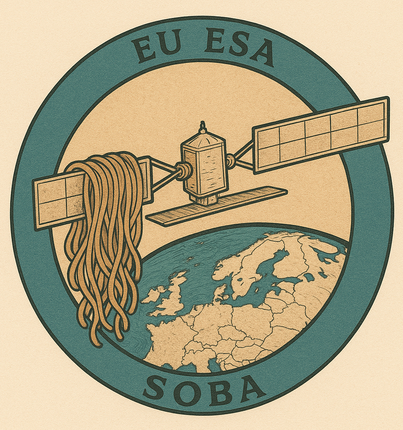
\includegraphics[width=0.4\textwidth]{logo_soba.png}

    \vspace{2cm}

    {\Huge \textbf{SOBA Project} \par}
    \vspace{1cm}
    {\Large \textbf{Technical documentation for @@DATASET_NAME@@ reference TEST dataset} \par}

    \vspace{2cm}

    \textbf{Work Package 3: Datasets Preparation} \\
    \vspace{0.5cm}

    \begin{minipage}{0.85\textwidth}
        \textbf{Scope:} @@SCOPE_TEXT@@
    \end{minipage}

    \vfill

    \begin{center}
    \begin{tabular}{ll}
        \textbf{Document Version} & 1.0.0 \\
        \textbf{Date} & \DTMtoday \\
        \textbf{Authors} & SOBA consortium \\
        \textbf{Intended Audience} & internal \\
        \textbf{Project delivrable document identifier} & TN5 \\
    \end{tabular}
    \end{center}

    \vspace{1cm}
\end{titlepage}

\tableofcontents

\newpage

% Utilisation du diagramme avec légende

%\begin{figure}[htbp]
%    \centering
%    %documentclass[a4paper,landscape]{article}.txt
%\documentclass[a4paper,landscape]{article}
%\usepackage[margin=1cm]{geometry}
%\usepackage{tikz}

\usetikzlibrary{shapes.geometric, arrows, positioning, calc}

%\begin{document}

\pagestyle{empty}

\tikzset{
    input/.style = {rectangle, draw, fill=orange!30, text centered, minimum height=0.7cm, minimum width=2.2cm, rounded corners=2pt, align=center, font=\small\sffamily},
    tool/.style  = {rectangle, draw, fill=blue!30, text centered, minimum height=0.7cm, minimum width=2.2cm, rounded corners=2pt, align=center, font=\small\sffamily},
    dataset/.style = {rectangle, draw, fill=green!30, text centered, minimum height=0.7cm, minimum width=2.2cm, rounded corners=0pt, align=center, font=\small\sffamily},
    highlight/.style = {dataset, draw=red!90!black, thick, font=\small\sffamily\bfseries},  % <-- nouveau style
    arrow/.style = {thick, -stealth},
}

\begin{tikzpicture}[node distance=0.8cm and 1.5cm]

% ---- Entrées ----
\node[input] (A) {S-1 ESA products};
\node[input, below=0.8cm of A] (B) {APIs: CDSE, \\ EODMSRapids, \\ PODAAC SWOT};
\node[input, below=0.8cm of B] (C) {reference products\\ at Ifremer};

% ---- Outil de construction des matchups ----
\node[tool, right=1.5cm of A] (build_match) {tool to \\ build matchups};

\draw[arrow] (A) -- (build_match);
\draw[arrow] (B) -- (build_match);
\draw[arrow] (C) -- (build_match);
% ---- Dataset matchups ----
\node[dataset, right=1.8cm of build_match] (matchups) {matchups files};

\draw[arrow] (build_match) -- (matchups);

% ---- Branche 1 : co-aligned -> split -> test (à gauche) ----
% Départ diagonal vers le bas-gauche (angle 225°)
\node[tool, below left=2.2cm and 1.0cm of matchups] (coalign) {tool to \\ build co-aligned};
\node[highlight, below=0.8cm of coalign] (coaligned_dataset) {co-aligned parquet};  % <-- style highlight
\node[tool, below=0.8cm of coaligned_dataset] (split) {tool to \\ split co-aligned};
\node[dataset, below=0.8cm of split] (splitout) {splited listings};
\node[tool, below=0.8cm of splitout] (gentest) {tool to \\ build test};
\node[dataset, below=0.8cm of gentest] (test) {test dataset};

\draw[arrow] (matchups.south) -- (coalign.north); % diagonale directe

\draw[arrow] (coalign) -- (coaligned_dataset);
\draw[arrow] (coaligned_dataset) -- (split);
\draw[arrow] (split) -- (splitout);
\draw[arrow] (splitout) -- (gentest);
\draw[arrow] (gentest) -- (test);

% ---- Branche 2 : co-locations -> training -> train & val (à droite) ----
% Départ diagonal vers le bas-droit (angle 315°)
\node[tool, below right=2.2cm and 1.0cm of matchups] (coloc_builder) {tool to \\ build co-locations};
\node[dataset, below=0.8cm of coloc_builder] (coloc) {co-locations};
\node[tool, below=0.8cm of coloc] (train_builder) {tool to \\ build training};
\node[dataset, below left=0.6cm and 0.5cm of train_builder] (train) {train dataset};
\node[dataset, below right=0.6cm and 0.5cm of train_builder] (val) {val dataset};

\draw[arrow] (matchups.south) -- (coloc_builder.north);

\draw[arrow] (coloc_builder) -- (coloc);
\draw[arrow] (coloc) -- (train_builder);
\draw[arrow] (train_builder) -| (train);
\draw[arrow] (train_builder) -| (val);

% ---- Jonction entre les branches : lien de splitout vers coloc_builder ----
\draw[arrow] (splitout) -- (coloc_builder);

\end{tikzpicture}

%\end{document}
%    \caption{SOBA Dataflow schema}
%    \label{fig:dataflow}
%\end{figure}

\section*{Version History}
\addcontentsline{toc}{section}{Version History}

\begin{table}[H]
    \centering
    \caption{Versioning of the documentation}
    \label{tab:versioning_documentation}
    \begin{tabular}{@{}p{2cm}p{3cm}p{8cm}p{4cm}@{}}
        \toprule
        \textbf{Version} & \textbf{Date} & \textbf{Modification} & \textbf{Author} \\
        \midrule
        1.0.0 & \DTMtoday & Creation of the HSCAT TEST dataset document & Ilias Reguig \\
        \bottomrule
    \end{tabular}
\end{table}

\begin{table}[H]
    \centering
    \caption{Versioning of test catalogue files}
    \label{tab:versioning_catalogue_files}
    {\small
    \begin{tabular}{@{}>{\raggedright\arraybackslash}p{7cm}p{2cm}>{\raggedright\arraybackslash}p{7cm}@{}}
        \toprule
        \textbf{File name} & \textbf{Date} & \textbf{Modifications} \\
        \midrule
        @@FILE_VERSION_ROW@@
        \bottomrule
    \end{tabular}
    }
\end{table}

\newpage

% ---------------------------
% SECTION 1 : Dataset Content Description
% ---------------------------

\section{Dataset Content Description}
\textbf{Dataset general description:} @@GENERAL_DESCRIPTION@@

\subsection{Global Coverage Map}
\textbf{Description:} @@COVERAGE_DESCRIPTION@@
\begin{figure}[H]
    \centering
    \includegraphics[width=\textwidth]{@@COVERAGE_FIGURE@@}
    \caption{@@COVERAGE_CAPTION@@}
    \label{fig:coverage_map}
\end{figure}

\subsection{Monthly Distribution of Matchups}
\textbf{Description:} @@MONTHLY_DESCRIPTION@@
\begin{figure}[H]
    \centering
    \includegraphics[width=0.85\textwidth]{@@MONTHLY_FIGURE@@}
    \caption{@@MONTHLY_CAPTION@@}
    \label{fig:monthly_distribution}
\end{figure}

\subsection{Reference Parameter Distribution}
\textbf{Description:} @@REFERENCE_DESCRIPTION@@
\begin{figure}[H]
    \centering
    \includegraphics[width=\textwidth]{@@WINDSPEED_FIGURE@@}
    \caption{@@REFERENCE_CAPTION@@}
    \label{fig:ref_distribution}
\end{figure}

Table~\ref{tab:reference_stats} summarises the retained HSCAT wind speeds.
@@REFERENCE_STATS_TABLE@@

\subsection{Catalogue Columns}
Table~\ref{tab:columns} lists every column of the reference TEST dataset, grouped by role.
\begin{longtable}{@{}p{4.1cm}p{1.9cm}p{8.6cm}@{}}
    \caption{Columns of the reference TEST dataset.\label{tab:columns}} \\
    \toprule
    \textbf{Column} & \textbf{Type} & \textbf{Description} \\
    \midrule
    \endfirsthead
    \toprule
    \textbf{Column} & \textbf{Type} & \textbf{Description} \\
    \midrule
    \endhead
    \bottomrule
    \endlastfoot
@@TEST_COLUMNS@@
\end{longtable}

@@SAMPLING_NOTE@@

\subsection{Global Metadata}
The five global attributes below are stored in both the TEST and TARGET Parquets.
\begin{longtable}{@{}p{5.4cm}p{8.9cm}@{}}
    \caption{Global attributes of the TEST and TARGET files.\label{tab:metadata}} \\
    \toprule
    \textbf{Attribute} & \textbf{Value} \\
    \midrule
    \endfirsthead
    \toprule
    \textbf{Attribute} & \textbf{Value} \\
    \midrule
    \endhead
    \bottomrule
    \endlastfoot
@@METADATA_ROWS@@
\end{longtable}

\newpage
% ---------------------------
% SECTION 2 : Dataset Production Steps
% ---------------------------
\section{Dataset Production Steps}
\subsection{Selected Products}
@@SELECTED_PRODUCTS@@
\begin{itemize}
    \item \textbf{Input co-aligned datasets:}
    \begin{itemize}
@@SOURCE_FILES@@
    \end{itemize}
    \item \textbf{SAR acquisition mode:} WV
    \item \textbf{Polarization:} SV, as encoded in the catalogue names
\end{itemize}
\textbf{Reference Product:} @@REFERENCE_PRODUCT@@

\subsection{Selection of Tiles / Filtered Co-locations}
@@SELECTION_INTRO@@
\begin{enumerate}
    \item @@GEO_CRITERION@@
    \item @@TIME_CRITERION@@
\end{enumerate}
The primary key is @@KEY_FORMULA@@. TEST and TARGET contain identical ordered keys.

@@FILTER_INTRO@@
@@QUALITY_FILTER_TABLES@@

\textbf{Accepted rows by mission:}
\begin{table}[H]
    \centering
    \begin{tabular}{lr}
        \toprule
        \textbf{Mission} & \textbf{TEST rows} \\
        \midrule
@@MISSION_ROWS@@
        \midrule
        Total & @@ROW_COUNT@@ \\
        \bottomrule
    \end{tabular}
\end{table}

\textbf{Excluded rows after the quality filters (key, required fields, duplicate):}
\begin{table}[H]
    \centering
    \begin{tabular}{lr}
        \toprule
        \textbf{Reason} & \textbf{Rows} \\
        \midrule
@@EXCLUSION_ROWS@@
        \bottomrule
    \end{tabular}
\end{table}

\textbf{Processing Steps:}
\begin{enumerate}
@@PROCESS_STEPS@@
\end{enumerate}

\subsection{Libraries and Commands Used}
@@COMMAND_INTRO@@
\begin{lstlisting}[caption={Command used to generate this dataset.}, label={lst:code}]
@@COMMAND@@
\end{lstlisting}

\subsection{Configuration Files}
@@CONFIG_INTRO@@
\begin{lstlisting}[caption={Settings recorded for this dataset.}, label={lst:config}]
@@RUN_CONFIG@@
\end{lstlisting}

\newpage
% ---------------------------
% BIBLIOGRAPHIE
% ---------------------------
\newpage
\addcontentsline{toc}{section}{References}

\begin{thebibliography}{9}

\bibitem{soba_format}
SOBA Consortium.
\textit{Format Description for parquet co-aligned datasets}.
Technical Document, Ifremer / Galeio, 2026.
Available at: \url{https://docs.google.com/document/d/1h4bLs1Z67MLL5ws3ckL2zrdYkajXCRGQKpSfnLGABes/edit?usp=sharing}

\end{thebibliography}

\end{document}
